\documentclass[11pt]{article}
\usepackage[margin=1in]{geometry}
\usepackage{amsmath,amssymb,amsthm}
\usepackage{graphicx}
\usepackage{booktabs}
\usepackage{hyperref}
\usepackage[T1]{fontenc}
\usepackage{newtxtext,newtxmath}
\usepackage{enumitem}
\usepackage{csquotes}
\MakeOuterQuote{"}
\emergencystretch=2.5em
\sloppy

\hypersetup{colorlinks=true, linkcolor=blue, citecolor=blue, urlcolor=blue}

\title{ElasticMLA: Context-Aware Token-Wise Latent Capacity Allocation for Multi-Head Latent Attention}
\author{ElasticMLA Project}
\date{}

\begin{document}
\maketitle

\begin{abstract}
Multi-head Latent Attention (MLA) reduces autoregressive key-value (KV) cache storage by caching a compressed latent vector instead of per-head keys and values, but it assigns the same latent width to every token. We recast token-wise latent width as an \textbf{operational, basis-dependent rate allocation problem}: persistent cache bytes are provably affine in the sum of token rates, and upper-tail future-loss risk induces a formally ordered spectrum of safe rates between a token's average and worst reuse offset (Risk-Capacity Ordering, proved here). We implement a variable-width packed MLA cache with token-specific nested latent prefixes, offsets, ranks, and channel-order metadata, and a layer-0-full contextual router trained with a straight-through joint-rollout surrogate for the corresponding rate-penalized Lagrangian. On 30.6M-, 122.1M-, and 249.3M-parameter MLA language models (an 8x parameter range), we measure the full risk-capacity spectrum (not only mean and max): required rate rises monotonically from 9.00\%/8.22\%/7.15\% of the full latent width at the mean criterion to 74.07\%/72.92\%/76.03\% at the worst-offset criterion, with an almost scale-invariant normalized tail-capacity premium (0.651/0.647/0.689 at 30M/122M/250M). Diagnostic decomposition shows this separation reflects \textbf{pervasive cancellation across the reuse horizon, not rare catastrophic tokens}: over 93\% of mean-safe positions at every scale still have at least one future offset exceeding the loss budget, and the positive-part mean loss is roughly double the signed mean. This risk-capacity result is scale-consistent, robust, and does not depend on the router at all.

The routing result is more intricate, and we report it in full rather than selectively. The frozen, pre-registered router beats a random matched-budget allocation on 24 untouched sequences at 30M (-0.0196 nat, 95\% CI [-0.0291,-0.0094]) and 122M (-0.0325 nat, CI [-0.0458,-0.0196]), but with the same coarse tier grid used at 30M, the identical protocol fails outright at 250M (+0.0019 nat, CI includes zero). Because 30M used a coarse tier grid and 122M a fine one, this confounds scale with tier granularity; a second, independently pre-registered confirmation at 250M with a finer 18-tier grid \textbf{succeeds} (-0.0117 nat, CI excludes zero), showing the coarse-grid failure was substantially a tier-resolution artifact of our design, not purely a scale limitation. However, a separate, more robust comparison against simple \textbf{causal heuristic} baselines (absolute position, token identity, token rarity, token type), fit only on the original training/validation splits and evaluated at the identical byte budget, shows the router winning only 2 of 16 tested scale/tier/ heuristic combinations with a confidence interval excluding zero --- and losing more decisively with the \textit{finer} tier grid, because heuristics benefit from added resolution at least as much as the learned router does. We report this negative finding transparently across all four tested scale/tier configurations. The 122M and 250M-fine policies also miss their own +0.15-nat validation-time quality budgets on fresh data, independently of the allocation result. Overall, this work provides a formal rate-allocation framework, a scale-consistent risk-capacity finding, and a rigorously audited routing method whose advantage over pure random allocation is real but tier-grid-dependent, and whose advantage over simple non-learned heuristics is not established at any tested configuration. A direct T4 GPU benchmark additionally shows a modest measured peak-memory reduction (3.5-4.2\%) alongside a severe measured decode-latency cost (168-201x slower than full MLA), traced to an unvectorized Python-loop cache reconstruction that must be fixed before any serving benefit is possible.
\end{abstract}

\section{Introduction}

Autoregressive transformer inference stores a key and value representation for each past token in each attention layer. This KV cache grows linearly with context length, batch size, layer count, and attention width, and increasingly constrains serving capacity. Multi-head Latent Attention (MLA), introduced in DeepSeek-V2 [2] and retained in DeepSeek-V3 [3], addresses this cost by caching a shared low-dimensional latent representation and reconstructing per-head content keys and values when needed. Related work converts pretrained multi-head or grouped-query attention models to MLA [4] and combines low-rank attention with layer sharing or quantization [5].

Existing MLA designs nevertheless use one fixed latent width for all tokens. This is conservative if difficult tokens are rare: the width must accommodate tail cases even when most cached states can tolerate stronger compression. Conversely, naïve average-capacity routing can fail because a small number of under-provisioned tokens may affect many future predictions. This tension raises three questions:

\begin{enumerate}

\item Does token-level latent capacity vary under a future-loss criterion, and does the pattern replicate across model scales?

\item Can a router use contextual hidden states to place capacity better than a noncontextual policy at exactly the same persistent-cache tensor-payload byte budget?

\item Can token-wise ranks be represented as actual packed storage rather than only simulated by a dense mask?

\end{enumerate}

We answer these questions with \textbf{ElasticMLA}, a correctness-first prototype for token-specific MLA latent widths. The core design preserves a full-width first layer, predicts one discrete tier from the resulting contextual state, and shares the selected tier across downstream layers. This makes the routing decision contextual while avoiding the circular requirement of compressing the state needed to decide its own capacity.

Our contributions are:

\begin{itemize}

\item a genuine variable-width packed latent cache with token-level ranks and verified dense/full-rank equivalence;

\item a formal rate-allocation theory (Section 3.2) proving an exact cache-byte identity and a risk-capacity ordering across upper-tail loss criteria, and a corrected, provenance-tracked future-loss intervention that measures the resulting risk-capacity spectrum at three scales spanning an 8x parameter range (30M-250M);

\item a joint-rollout straight-through router objective that optimizes hard deployment tiers while regularizing expected rank;

\item a pre-specified, untouched 24-sequence-per-scale confirmation against exact-byte static and matched-histogram shuffle controls at four scale/tier-grid configurations, together with a diagnostic experiment that isolates tier granularity from model scale as a cause of one configuration's failure; and

\item a comparison against simple, non-learned causal heuristics that the random/shuffle controls alone would miss, plus a direct GPU benchmark of persistent cache bytes, peak memory, and decode latency.

\end{itemize}

The risk-capacity spectrum (contribution 2) is the paper's most robust finding: it is scale- consistent and does not involve the router. The routing contribution is narrower and more mixed, and we report it as such rather than rounding it up: contextual allocation beats \textit{random} matched-budget placement at 30M and 122M, and at 250M once tier resolution is matched to 122M's scheme, but we do not find it reliably beats simple hand-designed \textit{heuristic} placement at any scale or tier grid we tested. We do not claim optimized serving speed, lower peak memory beyond the small measured effect in Section 5.5, or a reliably calibrated quality constraint at every scale.

\section{Background and Related Work}

\subsection{Multi-head Latent Attention}

For hidden state $h_t$, MLA computes a compressed KV latent

\[c_t = W_{DKV}h_t \in \mathbb{R}^{d_c},\]

then reconstructs content keys and values using $W_{UK}c_t$ and $W_{UV}c_t$. A separate rotary key $k_t^R \in \mathbb{R}^{d_R}$ carries positional information. A fixed-width MLA cache stores $(c_t,k_t^R)$ instead of per-head K/V tensors. For sequence length $T$, $L$ layers, and element size $b$, its leading storage term is

\[M_{\text{MLA}} = bTL(d_c+d_R).\]

DeepSeek-V2 reports substantial KV-cache reduction and throughput gains from this representation [2]. MHA2MLA [4] and TransMLA [6] study converting existing architectures to MLA. These works motivate latent compression but do not directly establish token-wise variable-width storage.

\subsection{KV-cache compression and adaptive allocation}

KV-cache compression includes eviction, quantization, low-rank approximation, cross-layer sharing, and sparse attention. Cross-Layer Latent Attention combines several axes and reports aggressive compression [5]. Such methods show that cache states contain redundancy, but a global compression rate can conceal variation across positions. ElasticMLA differs by allocating a nested latent prefix to every token while retaining all token positions.

Dynamic allocation is challenging because quality depends jointly on many cached states. An isolated token intervention gives useful sensitivity labels but is not a joint-rollout oracle. Our early supervised routers exposed this mismatch: high accuracy on isolated mean-risk labels collapsed toward the smallest tier during simultaneous compression. This negative result motivates direct optimization under the deployed hard-routing rollout.

\subsection{Relation to token-conditioned and layer-wise MLA variants}

Closest in spirit is EG-MLA [7], which gates latent content per token via an embedding-conditioned mechanism, and CARE [8], which allocates rank across layers using covariance-aware decomposition. ElasticMLA differs along three axes simultaneously: (i) it changes the \textit{persistent cache width} itself through a genuinely packed, ragged representation rather than a fixed-width gate; (ii) the routing decision is trained end-to-end with a straight-through hard-tier joint-rollout surrogate under an explicit rate penalty, rather than a fixed heuristic or layer-only allocation; and (iii) we evaluate it against random, shuffled, \textit{and} causal-heuristic exact-byte controls, exposing a result those comparisons alone would miss: the router does not consistently beat simple hand- designed rules (Section 5.4). We see this combination --- runtime per-token packed rate allocation, joint hard-routing optimization, and honest heuristic comparison --- as the paper's main empirical novelty, while acknowledging that "learn an importance signal, then spend a discrete resource budget nonuniformly" is a general pattern shared with adaptive-computation and mixture-of-experts routing more broadly.

\section{Method}

\subsection{Nested latent prefixes and packed storage}

For each layer $\ell$, calibration produces a permutation $\pi_\ell$ of the $d_c$ latent channels using gradient-times-activation importance. A token assigned rank $r_t$ stores the nested prefix

\[\tilde c_{\ell,t}=c_{\ell,t}[\pi_\ell(1:r_t)].\]

The persistent representation contains a values buffer, int32 offsets, int16 ranks, an int16 channel permutation, and the decoupled RoPE key. For the evaluated batch-one configurations, its exact cache tensor-payload byte count is

\[M_{\text{packed}}=
b\left[Td_c+(L-1)T\bar r+TLd_R\right]
+4L(T+1)+2LT+2Ld_c,\]

where $\bar r=T^{-1}\sum_t r_t$. The final three terms count int32 offsets, int16 ranks, and int16 channel permutations. The implementation uses $b=4$. This excludes allocator rounding, framework-object overhead, router weights, and workspace memory. During attention, the prototype reconstructs a dense temporary latent tensor; the metric is therefore neither process/device memory nor a peak-memory or kernel-latency measurement.

\subsection{Terminology and two propositions}

We deliberately avoid calling $r_t$ an intrinsic matrix rank. Because MLA's latent coordinates can be rotated while compensating the up-projections ($c\mapsto Qc$, $W_U\mapsto W_UQ^{-1}$ for invertible $Q$), a coordinate-wise nested prefix is \textbf{basis dependent}: full-model equivalence under $Q$ does not imply prefix-code equivalence. This basis dependence echoes prior evidence that MLA's latent coordinates separate reusable content from position-specific information in a way that is sensitive to how the latent basis is analyzed [9]. We therefore call $r_t$ an operational retained- coordinate rate in the calibrated nested codebook $P_{\ell,r_1}\preceq\cdots\preceq P_{\ell,d_c}=I$.

\textbf{Proposition 1 (exact budget affinity).} From the byte formula above, for any two per-sequence rate allocations $\mathbf r,\mathbf s$ with the same downstream rank sum, $M_{\text{packed}}(\mathbf r)=M_{\text{packed}}(\mathbf s)$; more generally $M_{\text{packed}}(\mathbf r)-M_{\text{packed}}(\mathbf s)=b(L-1)\sum_t(r_t-s_t)$. This licenses exact-byte controls: any two allocations with equal rank sums have identical cache tensor-payload bytes.

Let $\Delta_{t,j}(r)=\ell_{t+j}(P_rc_t)-\ell_{t+j}(c_t)$ be the signed loss change at future offset $j\in\{0,\ldots,H-1\}$ from truncating only source token $t$ to rate $r$, and for tail count $k$ let $A_{t,k}(r)$ be the mean of the $k$ largest $\Delta_{t,j}(r)$ (so $k=H$ is the signed mean and $k=1$ is the maximum). Define the conservative suffix-safe rate $r^*_{t,k}(\epsilon)=\min\{r\in\mathcal R: A_{t,k}(r')\le\epsilon\ \forall r'\ge r\}$.

\textbf{Proposition 2 (risk-capacity ordering).} If $k_1\ge k_2$ then $A_{t,k_1}(r)\le A_{t,k_2}(r)$ for every $r$, hence $r^*_{t,k_1}(\epsilon)\le r^*_{t,k_2}(\epsilon)$. \textit{Proof.} The mean of the top-$k$ elements of a fixed vector cannot decrease as $k$ shrinks, so the suffix-feasible rank set for $k_2$ is a subset of that for $k_1$; their minima are ordered. This holds for any realized loss vector, including the empirically nonmonotone rank-loss curves we observe, and requires no assumption about the sign or shape of $\Delta_{t,j}$. It is what licenses reporting an ordered risk-capacity spectrum (Section 5.1) rather than only two endpoints.

Under a bounded-Lipschitz assumption on the future logit map, nested-prefix truncation additionally admits the sensitivity envelope $|\Delta_{t,j}(r)|\le\sqrt2K_{t,j}\|e_t(r)\|_2$, where $e_t(r)$ is the discarded latent tail and $K_{t,j}$ a local Lipschitz constant; this gives a monotone safety bound consistent with, but not proving, the realized risk-capacity ordering. Full derivations, the constrained joint rate-distortion formulation that motivates the router objective, a formal statement of the straight-through surrogate's scope, and further falsifiable predictions are given in \texttt{notes/\allowbreak theory\_contextual\_tail\_rate.md}.

\subsection{Corrected future-loss capacity analysis}

For each source position $p$ and candidate rank $r$, we simultaneously zero channels outside the layer-specific nested prefix at position $p$ in every layer; all other positions remain full rank. Let $\delta_{p,j}(r)$ denote the resulting change in next-token cross-entropy at future-loss offset $j\in\{0,\ldots,H-1\}$. We define

\[A_{p,\mathrm{mean}}(r)=\frac{1}{H}\sum_{j=0}^{H-1}\delta_{p,j}(r),\qquad
A_{p,\mathrm{max}}(r)=\max_{0\le j<H}\delta_{p,j}(r),\]

and, for $A\in\{\mathrm{mean},\mathrm{max}\}$,

\[r^*_{p,A}=\min\{r\in\mathcal R:
A_p(r')\le\epsilon\;\text{for every}\;r'\in\mathcal R,\;r'\ge r\}.\]

The suffix condition guards against nonmonotone rank-loss curves. We report the mean of $r^*_{p,A}$ over 768 probed positions, separately for the mean- and maximum-over-horizon criteria, with $H=32$ and $\epsilon=0.10$ nat. Version 4 fixes an earlier off-by-one error by including \texttt{logits[p]}, the first prediction affected by masking source position $p$. Calibration repeats, calibration windows, and evaluation windows are nonoverlapping. Each scale uses 24 sequences and 32 probed positions per sequence, with checkpoint, data, source, and record hashes stored for audit.

\subsection{Contextual router}

Layer 0 runs at full rank. Let $z_t$ be the normalized pre-attention state entering layer 1 after the layer-0 contextual update. A two-layer MLP router produces tier logits

\[a_t=g_\theta(z_t), \qquad r_t\in\mathcal T.\]

The selected tier is shared by all downstream layers. The 30M and 250M-coarse policies use a 4-tier grid at 6.25\%/25\%/62.5\%/100\% of $d_c$ ($\{16,64,160,256\}$ at 30M, $\{32,128,320,512\}$ at 250M). The 122M and 250M-fine policies use an 18-point grid from 16 to $d_c$ with 16-step spacing up to 64 and 32-step spacing thereafter (14 tiers at 122M's $d_c=384$, 18 tiers at 250M's $d_c=512$).

\subsection{Joint-rollout training}

Deployment uses the hard one-hot choice $y_t=\text{onehot}(\arg\max a_t)$. During training we use the straight-through estimator

\[\hat y_t = y_t + p_t-\operatorname{stopgrad}(p_t),\quad
p_t=\operatorname{softmax}(a_t/\tau).\]

The forward pass therefore matches hard-tier inference, while gradients follow the soft probabilities. The frozen base language model is optimized only through the router objective

\[\mathcal J(\theta)=\mathcal L_{LM}(\hat y)+\lambda\frac{1}{Td_c}
\sum_t\sum_{k}p_{t,k}\mathcal T_k.\]

The base model receives no gradients. Candidate $\lambda$ values are trained on 16 sequences and selected on four validation sequences. The selection rule chooses the minimum-byte candidate within a +0.15-nat validation loss budget that also beats an exact-byte static control. The chosen policies are $\lambda=0.4$ at 30M, $\lambda=0.8$ at 122M, $\lambda=0.4$ at 250M-coarse, and $\lambda=0.8$ at 250M-fine; the two 250M policies are trained and frozen independently to disentangle tier granularity from scale (Section 5.2). The 122M and 250M-fine routers use random router initialization; the others initialize from the isolated-position supervised router. Four older development sequences were repeatedly observed during method development and are treated only as exploratory; they are not used for any confirmatory claim.

\subsection{Exact-byte controls}

For the primary static control, let the router's downstream rank sum on one sequence be $R$. Writing $R=qT+m$, the control assigns rank $q+1$ to $m$ random positions independently of token content and rank $q$ to all others. Twenty allocations are averaged. It has exactly the same downstream rank sum and cache tensor-payload bytes as the router, while approximating a continuous uniform rank. This placement is position-independent only after borrowing the router's content-dependent realized budget for that sequence; it is not a globally fixed-budget policy.

The secondary control permutes the router's exact tier histogram across positions 20 times. It preserves both the cache tensor-payload byte budget and the marginal tier distribution, isolating whether contextual rank placement matters.

\section{Experimental Setup}

\subsection{Models and data}

We train three decoder-only MLA language models on TinyStories-tokenized data, spanning an 8x parameter range.

\begin{table}[t]
\centering
\resizebox{\textwidth}{!}{%
\small
\begin{tabular}{crrrrrrrr}
\toprule
Model & Parameters & Layers & $d_{model}$ & Heads & $d_c$ & $d_R$ & Context & Training tokens seen \\
\midrule
MLA-30M & 30.6M & 6 & 384 & 6 & 256 & 32 & 256 & 24.576M sampled tokens \\
MLA-122M & 122.14M & 12 & 768 & 12 & 384 & 32 & 384 & 147.46M tokens \\
MLA-250M & 249.27M & 16 & 1024 & 16 & 512 & 32 & 384 & 288M sampled tokens \\
\bottomrule
\end{tabular}
}
\end{table}

The 30M model was trained for 3,000 steps from an approximately 8.8M-token training corpus and its checkpoint has validation loss 1.9618. The 122M and 250M models share byte-identical held-out validation streams (same TinyStories corpus construction, seed, and split fraction) despite their different architectures. The 122M final step-8,000 checkpoint has validation loss 1.5662; the best logged value, 1.5179 at step 7,250, was not checkpointed. The 250M model was trained for 3,000 steps and reached validation loss 1.6588. We make no best-checkpoint claim for any model: all three use the final training step. 30M was trained locally (Apple Silicon MPS); 122M and 250M were trained on Kaggle (Tesla P100).

\subsection{Confirmation protocol}

Commit \texttt{a4bcc7f} established a manifest-based pre-registration protocol: before viewing any fresh-window result, we commit each policy's file, SHA-256 hash, the deterministic sampling seed (91,827), 24 fresh sequences, 20 control permutations, the primary endpoint, and the success rule to \texttt{experiments/\allowbreak fresh\_confirmation\_manifest.json}. Every scale/tier-grid configuration we report (30M, 122M, 250M-coarse, 250M-fine) has its own manifest entry frozen before its confirmation run; the 250M-fine entry, added after diagnosing the 250M-coarse tier-granularity confound, follows the identical procedure rather than a relaxed one. Fresh windows are sampled from the held-out evaluation region and separated from all 24 prior oracle/development windows and from one another by at least \texttt{block\_size + 1} tokens. The primary endpoint is paired per-sequence router loss minus mean exact-byte static loss. A configuration passes when the upper bound of its 95\% sequence-cluster bootstrap interval is below zero. We also report exact one-sided paired sign-flip tests and sequence win counts. \texttt{experiments/\allowbreak audit\_fresh\_confirmation.py} independently reconstructs the seeded sampler and recomputes every statistic from the raw per-sequence rows before a result is treated as valid; \texttt{experiments/\allowbreak audit\_joint\_training\_replay.py} additionally verifies that a from-scratch retrain reproduces the frozen policy bit-for-bit.

\section{Results}

\subsection{The full risk-capacity spectrum is monotone and nearly scale-invariant across 30M-250M}

We extend the two-point mean/max analysis to a full upper-tail spectrum computed from the same corrected, provenance-tracked windows, now at \textbf{three} scales spanning an 8x parameter range: for each source position we retain the largest $k$ of the $H=32$ future loss deltas, for $k\in\{32,16,8,4,2,1\}$, and take the smallest suffix-safe rank.

\begin{table}[t]
\centering
\small
\begin{tabular}{rrrrr}
\toprule
$k$ (of 32) & $\alpha=1-k/H$ & 30M $/d_c$ & 122M $/d_c$ & 250M $/d_c$ \\
\midrule
32 (mean) & 0.000 & 9.00\% & 8.22\% & 7.15\% \\
16 & 0.500 & 21.47\% & 23.00\% & 22.53\% \\
8 & 0.750 & 39.65\% & 39.52\% & 40.14\% \\
4 & 0.875 & 55.75\% & 54.22\% & 57.23\% \\
2 & 0.938 & 66.94\% & 65.56\% & 69.18\% \\
1 (max) & 0.969 & 74.07\% & 72.92\% & 76.03\% \\
\bottomrule
\end{tabular}
\end{table}

Every step is monotone nondecreasing at all three scales, exactly as Proposition 2 (risk-capacity ordering) guarantees. The normalized \textbf{tail-capacity premium} $\mathrm{TCP}=\mathbb E[r^*_{\max} -r^*_{\mathrm{mean}}]/d_c$ is 0.6507 (95\% CI [0.6335, 0.6673]) at 30M, 0.6470 (CI [0.6283, 0.6641]) at 122M, and 0.6888 (CI [0.6647, 0.7129]) at 250M --- three overlapping-to-adjacent intervals across an 8x parameter range, making this the most scale-consistent quantitative result in the paper.

\textbf{The separation is driven by pervasive cancellation, not rare catastrophic tokens, at all three scales.} At the rank that is safe under the signed mean criterion, the positive-part mean loss (mean of $\max(\Delta,0)$ over the horizon) is 2.05x (30M), 2.31x (122M), and 2.15x (250M) larger than the signed mean, and 93.1\%/94.1\%/96.1\% of such "mean-safe" positions still have at least one future offset whose loss increase exceeds $\epsilon$. If harm were concentrated in a few rare spikes, the vast majority of mean-safe positions would have zero offsets above $\epsilon$; instead nearly all of them do at every scale we tested, and the signed mean is kept small by cancellation against negative excursions elsewhere in the horizon. \textbf{Figure 2} (\texttt{figures/\allowbreak elasticmla\_risk\_spectrum.pdf}) shows the spectrum and this diagnostic across all three scales.

The 250M model (Section 4.1) contributes to the risk-capacity spectrum result here and, as described in Sections 5.2-5.4, to a full contextual-router replication under two different tier grids.

The normalized 122M-minus-30M difference in the original mean/max endpoints is -0.781 percentage points for the mean (95\% bootstrap CI: [-1.617, +0.076]) and -1.156 points for the maximum (CI: [-3.849, +1.611]); both include zero. This is not an equivalence test and does not establish scale invariance of the endpoints, but the tail-capacity premium result above is a stronger and separate scale-consistency finding computed across the whole spectrum and now three scales rather than two endpoints at two scales.

The per-record raw deltas underlying this spectrum were computed on ephemeral cloud job storage and are not independently re-auditable; only the aggregate summary (with verified checkpoint/data provenance) was recovered. See \texttt{notes/\allowbreak risk\_capacity\_spectrum\_results.md}.

\subsection{Fresh contextual routing beats exact-byte static allocation, with a tier-granularity dependence at 250M}

\begin{table}[t]
\centering
\resizebox{\textwidth}{!}{%
\small
\begin{tabular}{crrrrrrrc}
\toprule
Scale (tiers) & Mean rank & Packed / fixed MLA & $\Delta$loss vs full & Router - static & 95\% CI & Wins & Exact $p$ & Result \\
\midrule
30M (4 coarse) & 145.78 / 256 & 68.80\% & +0.1001 & \textbf{-0.01959} & [-0.02911, -0.00938] & 20/24 & 0.000655 & success \\
122M (14 fine) & 206.93 / 384 & 61.46\% & +0.1823 & \textbf{-0.03251} & [-0.04575, -0.01958] & 21/24 & 0.0000493 & success \\
250M (4 coarse) & 317.15 / 512 & 66.82\% & +0.1158 & +0.00190 & [-0.00222, +0.00610] & 13/24 & 0.806 & \textbf{failure} \\
250M (18 fine) & 278.67 / 512 & 60.19\% & +0.1659 & \textbf{-0.01165} & [-0.01911, -0.00394] & 17/24 & 0.00438 & success \\
\bottomrule
\end{tabular}
}
\end{table}

At 30M and 122M the router satisfies its separately pre-specified primary criterion. At 250M with the \textit{same} coarse 4-tier grid used at 30M, it does not: the point estimate is in the wrong direction and the CI includes zero. Because 30M used coarse tiers and 122M used a fine 14-tier grid, this coarse-only 250M result confounds scale with tier granularity, so we ran a second, independently pre-registered confirmation at 250M with an 18-tier fine grid (mirroring 122M's scheme; same base checkpoint, oracle, and channel orders; random router initialization, exactly as the 122M fine-grid policy was built). It \textbf{succeeds}: -0.01165 nat, CI excludes zero, p=0.0044. This shows the initial 250M failure was, at least in part, a tier-resolution artifact of our own design rather than purely an intrinsic scale limitation: at $d_c=512$, four coarse tiers are too low-resolution for the router to reliably beat random matched-budget allocation, but 18 finer tiers restore that advantage. We did not adjust either protocol after seeing its result; both were frozen in advance (\texttt{experiments/\allowbreak fresh\_confirmation\_manifest.json}, scale keys \texttt{250m} and \texttt{250m\_fine}), and we report both rather than only the more favorable one. Neither protocol pre-specified a family-wise multi-scale test, so we do not elevate these results to a single combined confirmatory claim; each frozen protocol stands on its own. Full detail: \texttt{notes/\allowbreak contextual\_router\_250m\_tier\_granularity\_diagnostic.md}.

The exact-histogram shuffle comparison is more forgiving at every scale/tier configuration we tested: router-minus-shuffle is -0.07989 nat at 30M (CI: [-0.08999, -0.06956]), -0.13907 nat at 122M (CI: [-0.15439, -0.12408]), -0.01765 nat at 250M-coarse (CI: [-0.02306,-0.01228]), and -0.03551 nat at 250M-fine (CI: [-0.04404,-0.02621]), with the router winning the large majority of sequences at every configuration. So within-sequence placement of the router's own chosen tier multiset consistently helps, even at the one configuration (250M coarse) where the overall rate selection does not beat random allocation.

\begin{figure}[t]

\centering

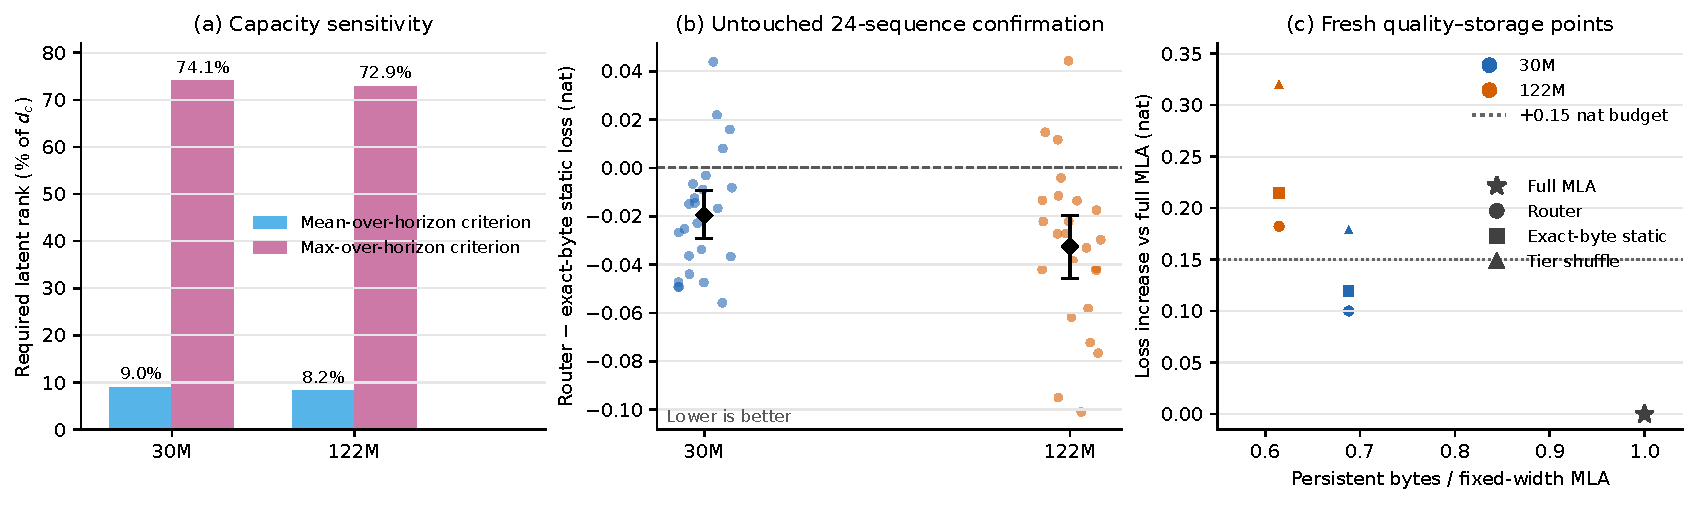
\includegraphics[width=\textwidth]{figures/elasticmla_main_results.pdf}

\caption{(a) Mean required rank under the mean- and maximum-over-32-token-horizon criteria, averaged over 768 probed positions per scale. (b) Per-sequence router-minus-control differences; dots are sequences, diamonds are means, and error bars are paired sequence-bootstrap 95\% intervals. (c) Mean fresh-sequence loss increases versus full MLA; both controls have exactly the router's per-sequence cache tensor-payload byte count. Points are discrete evaluated configurations, not an interpolated operating curve. Panel (a) shows only the mean/max endpoints; see Figure 2 for the full six-point risk-capacity spectrum. Panels (b)-(c) show only 30M/122M; see Section 5.2's table and \texttt{notes/\allowbreak contextual\_router\_250m\_tier\_granularity\_diagnostic.md} for both 250M configurations.}

\label{fig:elasticmla_main_results}

\end{figure}

\begin{figure}[t]

\centering


\includegraphics[width=\textwidth]{figures/elasticmla_risk_spectrum.pdf}

\caption{(a) Normalized suffix-safe rate against upper-tail level $\alpha=1-k/H$ at all three scales, with paired sequence-bootstrap 95\% bands; monotonicity is guaranteed by Proposition 2. (b) Signed mean, positive-part mean, and maximum loss delta at the rank that is safe under the signed mean criterion, annotated with the fraction of records having at least one future offset exceeding $\epsilon$; the gap between signed and positive-part means shows cancellation rather than rare spikes.}

\label{fig:elasticmla_risk_spectrum}

\end{figure}

\subsection{Quality-constraint generalization is imperfect, and is independent of the allocation result}

The 30M and 250M-coarse policies remain within the +0.15-nat selection budget on fresh sequences (fresh $\Delta$loss 0.1001 and 0.1158). The 122M and 250M-fine policies do not: validation $\Delta$loss was +0.1408 (122M) and +0.1483 (250M-fine), while fresh $\Delta$loss is +0.1823 (122M) and +0.1659 (250M-fine). Quality-budget calibration and allocation efficiency are separate axes and do not track each other: 122M keeps its allocation advantage over static despite missing its budget; 250M-coarse stays within budget yet loses its allocation advantage; 250M-fine regains the allocation advantage but also misses its budget. A deployable system should use a larger calibration set, a conservative risk margin, or online fallback to a higher tier for the quality-budget issue, and a fundamentally stronger training signal (Section 5.4, Section 6) for the allocation-advantage issue.

\subsection{The router does not reliably beat simple causal heuristics, at any scale or tier grid}

The random and matched-histogram-shuffle controls above are content-independent given the router's realized budget, but they are weak baselines: nothing prevents a simple, cheap, strictly causal rule (depending only on the current token and/or absolute position, never on future tokens or a sequence-global budget) from doing better. We fit four such rules --- absolute position, token identity (frequency-smoothed), inverse token rarity, and coarse token type --- using only the original 16 training sequences, select an additive rate bias on the original 4 validation sequences under the same +0.15-nat budget rule as the router, and evaluate once on the same 24 frozen fresh sequences at the router's own per-sequence byte budget.

\begin{table}[t]
\centering
\small
\begin{tabular}{ccrcc}
\toprule
Scale (tiers) & Control & Router - control (nat) & 95\% CI & Result \\
\midrule
30M (coarse) & position & +0.0138 & [0.0025, 0.0254] & \textbf{router loses} \\
30M (coarse) & lexical identity & -0.0253 & [-0.0399, -0.0114] & router wins \\
30M (coarse) & token rarity & -0.0268 & [-0.0412, -0.0124] & router wins \\
30M (coarse) & token type & +0.0065 & [-0.0042, 0.0174] & tie \\
122M (fine) & position & +0.0040 & [-0.0098, 0.0171] & tie \\
122M (fine) & lexical identity & +0.0067 & [-0.0044, 0.0177] & tie \\
122M (fine) & token rarity & +0.0468 & [0.0340, 0.0593] & \textbf{router clearly loses} \\
122M (fine) & token type & +0.0117 & [-0.0028, 0.0258] & tie \\
250M (coarse) & position & +0.0055 & [0.0011, 0.0097] & \textbf{router loses} \\
250M (coarse) & lexical identity & -0.0155 & [-0.0206, -0.0106] & router wins \\
250M (coarse) & token rarity & +0.0055 & [0.0010, 0.0098] & \textbf{router loses} \\
250M (coarse) & token type & +0.0055 & [0.0010, 0.0097] & \textbf{router loses} \\
250M (fine) & position & +0.0131 & [0.0020, 0.0254] & \textbf{router loses} \\
250M (fine) & lexical identity & +0.0557 & [0.0448, 0.0682] & \textbf{router clearly loses} \\
250M (fine) & token rarity & +0.0371 & [0.0252, 0.0501] & \textbf{router clearly loses} \\
250M (fine) & token type & +0.0612 & [0.0492, 0.0744] & \textbf{router clearly loses} \\
\bottomrule
\end{tabular}
\end{table}

At 250M-coarse, position, rarity, and type collapse to numerically identical results: with only four coarse tiers, their validation-selected bias saturates almost the entire sequence into a single mid-high tier, degenerating toward near-uniform allocation, and even that beats the router. At 250M-fine, giving every heuristic the same finer 18-tier resolution that let the router beat \textit{random} allocation (Section 5.2) makes the heuristics stronger too --- strong enough that \textbf{all four now beat the router}, including lexical identity, which had been the router's best result at every other configuration. Finer tiers help simple heuristics at least as much as they help the learned router.

Across all four scale/tier configurations (16 scale-control pairs), only two pairs show a router win with a CI excluding zero, both at 30M. \textbf{This is the paper's most durable negative finding}: contextual placement is sometimes better than \textit{random or shuffled} placement at equal bytes --- and whether it is depends on tier granularity, not simply model scale (Section 5.2) --- but current evidence does not show it is reliably better than simple hand-designed heuristics, at any of the four scale/tier-grid configurations we tested, coarse or fine, small or large model. We report this as an honest negative finding (\texttt{notes/\allowbreak causal\_heuristic\_baseline\_results.md}, \texttt{notes/\allowbreak contextual\_router\_250m\_tier\_granularity\_diagnostic.md}, \texttt{experiments/\allowbreak evaluate\_causal\_heuristic\_routers.py}) rather than omit it: it indicates that the isolated-position future-loss signal used to construct oracle labels, and the joint-rollout straight-through training that refines it, are not yet strong enough to reliably out-perform inexpensive non-learned rules, and simply changing tier resolution or model scale does not fix this on its own, motivating stronger joint objectives, larger calibration sets, or hybrid heuristic-plus-learned designs as future work.

\subsection{Measured GPU memory and latency confirm storage savings and reveal a severe latency cost}

Section 3.1's byte formula is a derived tensor-payload count. We additionally benchmarked real prefill-then-128-step incremental decode on a Tesla T4 GPU at both scales, comparing full-width dense MLA, a uniform packed cache matched to the router's realized rank, and the router's packed cache (\texttt{experiments/\allowbreak benchmark\_cache\_memory\_latency.py}).

\begin{table}[t]
\centering
\small
\begin{tabular}{crrr}
\toprule
Scale & Cache bytes (router / full) & Peak allocated (router / full) & Mean decode step (router vs full) \\
\midrule
30M & 67.4\% & 96.5\% & 1412.6 ms vs 8.41 ms (\textbf{167.9x slower}) \\
122M & 59.6\% & 95.8\% & 3592.9 ms vs 17.87 ms (\textbf{201.1x slower}) \\
\bottomrule
\end{tabular}
\end{table}

Measured cache-byte ratios closely track the derived formula. Peak allocated memory is modestly \textit{lower} for packed configurations (3.5-4.2\% at the router's realized rank), a small positive result we had not previously claimed. Decode latency, however, is two orders of magnitude worse for the packed path, because \texttt{pack\_latents}/\texttt{unpack\_latents} reconstruct the entire cached history with a per-token Python loop on every decode step --- an implementation limitation, not a property of the packed representation itself. See \texttt{notes/\allowbreak measured\_cache\_memory\_latency.md} for full results at both configurations (uniform and router) and both scales.

\section{Validity, Reproducibility, and Limitations}

\textbf{Statistical scope.} The unit of inference is a full sequence, not an individual token. Twenty- four clusters per scale support paired uncertainty estimates but remain modest. The exact sign-flip p-values enumerate all sign assignments conditional on the observed magnitudes, but their inferential interpretation still requires exchangeability of paired-difference signs under the null. The intervals and tests do not incorporate checkpoint, policy-seed, or training-run variability. We evaluate one checkpoint per scale, one data distribution, and one router seed. The per-record raw deltas underlying the risk-capacity spectrum (Section 5.1) were computed on ephemeral cloud job storage and could not be retrieved after job completion; only the aggregate summary statistics (independently checkpoint/data-hash verified) were recovered, so that spectrum is not re-auditable at the per-position level the way the confirmation results are.

\textbf{Threshold scope.} Raw rank-loss curves are frequently nonmonotone: 83.6\%/89.3\% of mean-over-horizon curves and 59.4\%/69.7\% of maximum-over-horizon curves at 30M/122M respectively (not separately re-measured at 250M, though the identical conservative suffix rule is applied there too). Accordingly, $r^*$ uses the conservative suffix rule and is defined only on the tested discrete rank grid; it should not be interpreted as a smooth or uniquely identified intrinsic rank.

\textbf{Control scope.} The primary control randomizes rank placement conditional on each router sequence's realized total rank; it is therefore position-independent, but not a globally fixed- budget policy. Twenty random allocations estimate its per-sequence loss. Section 5.4 adds four causal heuristic baselines (position, lexical identity, rarity, type) at the same realized budget across all four scale/tier-grid configurations (16 scale-heuristic comparisons); the router shows a confident win in only 2 of 16. We still lack a comparison against separately optimized global-budget static policies, a learned orthogonal (PCA/SVD) nested basis, and eviction/quantization baselines from the wider KV-cache compression literature.

\textbf{Oracle scope.} Capacity labels are isolated-position interventions, not joint-rollout-optimal labels. Joint training alleviates but does not solve this limitation.

\textbf{System scope (now measured, not only derived).} We benchmarked real prefill+128-step incremental decode on a Tesla T4 GPU at both scales (\texttt{experiments/\allowbreak benchmark\_cache\_memory\_latency.py}, \texttt{notes/\allowbreak measured\_cache\_memory\_latency.md}). Measured persistent cache bytes closely track the byte-formula predictions (67.2-67.4\% of full MLA at 30M, 54.2-59.6\% at 122M). Peak allocated GPU memory is modestly lower for packed configurations (1.3-4.2\% reduction), a small positive result we had not previously claimed. However, \textbf{decode latency is 168-201x slower} for the packed path than full-width dense MLA at both scales, because \texttt{pack\_latents}/\texttt{unpack\_latents} reconstruct the entire cached history with a per-token Python loop on every decode step. We therefore still do not claim any latency, throughput, or superiority to optimized MHA/GQA/FlashMLA kernels; on the contrary, we now have direct evidence that the current implementation is roughly two orders of magnitude too slow for real decoding, and identify the specific unvectorized code path responsible.

\textbf{Quality scope.} Every compressed policy increases loss relative to full MLA, and the 122M and 250M-fine policies miss their held-out +0.15-nat budget (30M and 250M-coarse do not). Task-level generation quality is not evaluated.

\textbf{Architecture scope.} Layer 0 is always full, and one tier is shared by every downstream layer. Per-layer routing could improve efficiency but increases metadata, training complexity, and kernel divergence.

\textbf{Reproducibility.} Result artifacts contain checkpoint/data/policy/source hashes and exact starts. A post-hoc audit reconstructs the pre-specified sampler, verifies nonoverlap, derives cache bytes from authenticated checkpoint dimensions, and recomputes all summary statistics. Deterministic training replays reproduce the frozen router tensors, histories, splits, and hyperparameters bit-for-bit. The original cloud commands preceded the later manifest-enforcement arguments; this is disclosed, and the frozen protocol commit plus complete logs and audits bind the original results. Future runs fail unless their manifest inputs match.

\section{Conclusion}

We formalize token-wise MLA latent width as a basis-dependent operational rate allocation problem: persistent cache bytes are exactly affine in summed token rates (Proposition 1), and upper-tail future-loss risk induces a provably monotone spectrum of safe rates between average and worst-case reuse (Proposition 2). Measured at 30M, 122M, and 250M (an 8x parameter range), this spectrum is nearly scale-invariant in its normalized tail-capacity premium (0.65-0.69 across all three scales) and shows that the mean/tail separation arises from pervasive cancellation across the reuse horizon rather than rare catastrophic tokens --- a mechanistic finding that revises the intuitive "rare spike" story and is the paper's most robust contribution, independent of the router.

The routing contribution requires two axes to describe honestly, both established through pre-registered, independently audited protocols rather than post-hoc adjustment. First, whether the router beats \textit{random} matched-budget allocation depends on tier granularity as well as scale: it succeeds with a coarse 4-tier grid at 30M and a fine 14-tier grid at 122M, fails with a coarse grid at 250M, and succeeds again at 250M once tier resolution is increased to match 122M's scheme --- so the initial appearance of a pure scale effect was substantially a tier-resolution confound in our own design, which we diagnosed and corrected rather than let stand. Second, and more importantly, whether the router beats simple \textbf{causal heuristics} (position, token identity, rarity, type) does \textit{not} depend favorably on tier granularity: across four tested scale/tier-grid configurations (16 scale-heuristic comparisons), the router wins with a confidence interval excluding zero in only 2 cases, and its losses become more numerous and more confident with the finer tier grid at 250M, because simple heuristics benefit from added resolution at least as much as the learned router does. We report both axes transparently rather than overclaim: the present evidence establishes a formal allocation framework, a scale-consistent risk-capacity spectrum, and a routing method with a real but tier-grid-dependent advantage over random placement and no established advantage over cheap non-learned heuristics at any tested configuration --- not peak-memory or latency gains (a direct T4 benchmark shows the packed path is 168-201x slower per decode step than full MLA despite modestly lower peak memory, because the packed cache reconstruction is an unvectorized Python loop), and not a reliably calibrated quality constraint at 122M or 250M-fine. Priority future work is (1) closing the gap to causal heuristics --- via joint-rollout-consistent oracle labels, distillation from the heuristics that currently win, tier- resolution-aware training, or hybrid heuristic-plus-learned designs --- before further scale-up is attempted, since scale alone does not fix this, (2) a grouped-tier or fused packed attention kernel to convert the established persistent-byte savings into measured peak-memory and latency gains against optimized MHA/GQA/MLA/FlashMLA baselines, and (3) replication across more seeds, domains, and larger, more realistically trained checkpoints once (1) is resolved.

\begin{thebibliography}{9}

\bibitem{ref1} A. Vaswani et al., "Attention Is All You Need," NeurIPS, 2017.

\bibitem{ref2} DeepSeek-AI, "DeepSeek-V2: A Strong, Economical, and Efficient Mixture-of-Experts Language Model," arXiv:2405.04434, 2024.

\bibitem{ref3} DeepSeek-AI, "DeepSeek-V3 Technical Report," arXiv:2412.19437, 2024.

\bibitem{ref4} T. Ji et al., "Towards Economical Inference: Enabling DeepSeek's Multi-Head Latent Attention in Any Transformer-based LLMs," arXiv:2502.14837, 2025.

\bibitem{ref5} "Lossless KV Cache Compression to 2\%" (Cross-Layer Latent Attention), arXiv:2410.15252, 2024.

\bibitem{ref6} "TransMLA: Multi-Head Latent Attention Is All You Need," arXiv:2502.07864, 2025.

\bibitem{ref7} "EG-MLA: Embedding-Gated Multi-head Latent Attention for Scalable and Efficient LLMs," arXiv:2509.16686, 2025.

\bibitem{ref8} "CARE: Covariance-Aware and Rank-Enhanced Decomposition for Enabling Multi-Head Latent Attention," arXiv:2603.17946.

\bibitem{ref9} "Through the Bottleneck: How Multi-head Latent Attention Separates Content from Position in Language Models," arXiv:2607.23054.

\end{thebibliography}

\end{document}
